\documentclass{article}
\usepackage{graphicx} % Required for inserting images
\usepackage{hyperref}
\usepackage[ruled,vlined]{algorithm2e}
\usepackage{pythontex} 

\title{Compte-rendu du projet d'analyse de données: applications au jeu Stardle}
\author{Charles Azais de Vergeron et Octave Feuilland }
\date{Mai 2025}

\begin{document}

\maketitle

\section{Introduction}
\subsection{Présentation du jeu Stardle}

Le jeu Stardle est un jeu en ligne (\href{https://stardle.net}{stardle.net}) basé sur le jeu Wordle / SUTO. 
Le but est de deviner chaque jour un vaisseau choisi au hasard parmi une liste d'environ 200 éléments.

Chaque vaisseau est definit par deux types de caractéristiques: 
\begin{itemize}
    \item Qualitatives
    \begin{itemize}
        \item Fabricant (Manufacturer)
        \item Type
        \item Role 
        \item Année d'apparition (Relese Date)
        \item En Jeu ou Non (Status)
    \end{itemize}
    \item Quantitatives
    \begin{itemize}
        \item Nombre de personnes dans l'équipage (Crew)
        \item Valeur en \$ (Price)
        \item Valeurs en monnaie du jeu (Price In game)
        \item Capacité en tant que cargo (Cargo Capacity)
        \item Vitesse de croisière (SCM) et maximale (Max)
        \item Longeur (Length), Largeur (Beam) et Hauteur (Height)
    \end{itemize}
\end{itemize}

Voici un exemple de partie du jeu : \\

\begin{figure}[h]
    \centering
    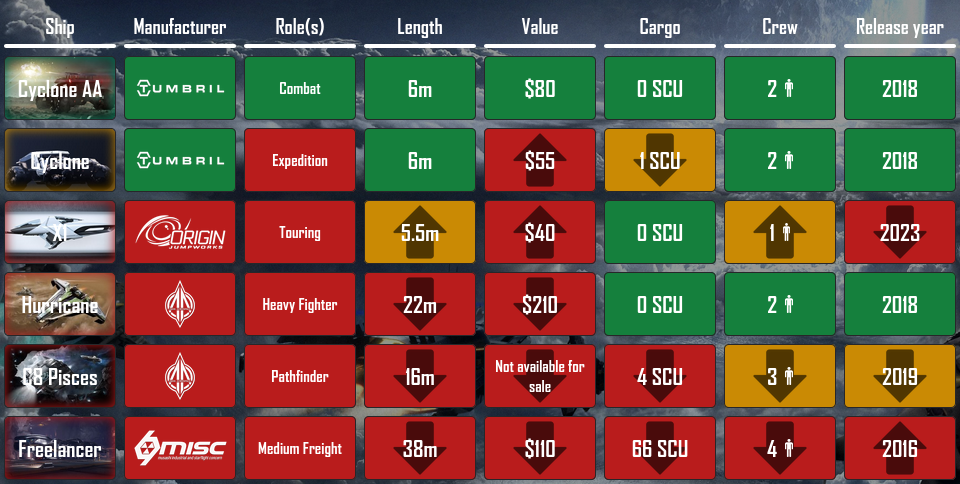
\includegraphics[width=0.8\textwidth]{stardle.png}
    \caption{Exemple de partie du jeu Stardle}
    \label{fig:stardle}
\end{figure}

Nous avons 3 possibilités de résultats: Vrai, Faux ou Proche (uniquement pour les caractéristiques quantitatives).
\subsection{Objectif du projet}

L'objectif de ce projet est d'analyser les données du jeu Stardle afin de créer un algorithme capable de trouver 
un vaisseau pris au hasard dans la base de données en un minimum de tentatives et de déterminer une combinaison 
d'essais de vaisseaux qui permet de minimiser le nombre de tentatives.

Nous avons donc récupéré les données et recréé le jeu puis essayé de trouver un 
algorithme optimal pour déterminer le vaisseau le plus efficacement possible.


\section{Récupération des données}
La récupération des données est faite via le script Python CreateShipDatabase.py. 
Ce script utilise l'API officielle de \href{https://starcitizen.tools/}{Star Citizen Wiki}  pour récupérer les informations sur les vaisseaux.

\subsection{Structure du script}
Le script se décompose en plusieurs étapes principales :

\begin{enumerate}   
    \item \textbf{Collecte des données} \\
    Nous utilisons l'API \verb|https://api.star-citizen.wiki/| pour obtenir la liste complète des 
    vaisseaux.
        Pour chaque vaisseau, le script récupère les données via l'API et 
        extrait toutes les caractéristiques -- dans la configuration "All" -- 
        et uniquement celles du jeu Stardle -- dans la configuration  "Stardle" --\\
        Dans la suite du rapport, "Stardle" désigne la configuration du jeu et "All" la configuration complète.
    \item \textbf{Stockage des données}
    
    \begin{itemize}
        \item Création de deux fichiers JSON :
        \begin{itemize}
            \item \verb|shipList.json| : liste des vaisseaux et leurs liens
            \item \verb|shipDB_All.json| : base de données complète des vaisseaux
            \item \verb|shipDB_Stardle.json| : base de données avec les catégories du jeu Stardle 
        \end{itemize}
    \end{itemize}
\end{enumerate}


\section{Nettoyage et préparation des données}

Pour ajouter de la complexité aux données d'origine, nous avons mélangé les deux bases de données.
Stardle est la base du projet. Nous avons extrait de All les valeurs de scm, max, length, beam. Nous avons aussi 
rajouté une colonne "price in game" qui correspond à la valeur du vaisseau dans le jeu.(via le site 
\href{https://www.erkul.games/live/calculator}{Erkul.com})\\

Pour la gestion des valeurs manquantes, nous avons étudié les dependances entre les colonnes.
Nous avons remarqué que certaines colonnes étaient très corrélées entre elles. Par exemple, le prix \$ (sans valeurs manquantes) 
et celle du prix en jeu (avec beaucoup des valeurs manquantes). Nous avons tenté de remplr les valeurs manquantes
en utilisant une regression lineaire et une regression quadratique mais ce ne fut pas concluant. 
Nous avons donc appliqué l'algorithme suivant: \\
\\

\begin{algorithm}[H]
    \SetAlgoLined
    \KwResult{Colonne sans valeurs manquantes}
    texte\\
    \For{texte}{
        Texte\;
        \eIf{condition}{
            texte\;
            texte\;
        }{
            texte;
        }
    }
    texte\;
    \caption{texte}
    \end{algorithm}


\section{Implementation du jeu}

Nous avons recréé le jeu Stardle en Python : \verb|stardle.py|
Nous avons commencé par afficher l'intégralité des vaisseux du jeu pour éviter au joueur de se tromper
lors de la saisie.
Nous reproduisons la meme logique que le jeu original
puis après nous avons à taper le nom du vaisseux. Ca affiche les résultats.

\section{Algorithme de jeu}

En suivant les sujets abordés en cours, nous avons décidé d'aborder le problème par la théorie des graphes.
Considérons les vaisseaux comme des nœuds, leurs types comme des arêtes par exemple (mais aussi leur rôle, fabricant...).
L'avantage du type est qu'un même vaisseau peut en avoir deux, ce qui crée plus de connexions qu'avec 
les fabricants par exemple.
Voici un exemple de graphe : 

\begin{figure}[h]
    \centering
    \includegraphics[width=1\textwidth]{graphe_type.png}
    \caption{Graphe des vaisseaux par type}
    \label{fig:graph}
\end{figure}


Nous étudions donc les vaisseaux du point de vue de la théorie des graphes sur les relations qualitatives 
(fabricant, type, rôle, année d'apparition, en jeu ou non).
Nous avons arbitrairement mis un poids de 1.0 à chaque différence qualitative pour pondérer les chemins 
entre vaisseaux. Cela nous donne le csv \verb|path_history.csv|. Avec ce csv, nous pouvons déterminer les éléments 
voisins et ainsi directement les sélectionner pour les prochaines étapes de l'algorithme.

\subsection{Algorithme de Stardle}
\begin{algorithm}[H]
\SetAlgoLined
\KwData{base de données des vaisseaux}
\KwResult{Vaisseau inconnu trouvé}

\;
\;
\For{chaque vaisseau dans la liste}{
    Requête GET pour obtenir les détails du vaisseau\;
    \eIf{DataBaseType == "Stardle"}{
        Extraire: nom, fabricant, rôle, longueur, prix, cargo, équipage\;
        Ajouter au ShipDB\;
    }{
        Sauvegarder toutes les données du vaisseau\;
    }
}
Sauvegarder ShipName dans shipList.json\;
Sauvegarder ShipDB dans shipDB\_[Type].json\;
\caption{Récupération des données des vaisseaux}
\end{algorithm}


\end{document}